\todo[inline]{Переделать верстку}

Электрический ток представляет собой направленный перенос зарядов. Микрочастицы, осуществляющие этот перенос, называют \important{носителями тока}. В простейшем случае (ток в вакуумном диоде, ионный пучок в масс-спектрометре, и т.~д.) носителями тока являются заряженные частицы, движущиеся в свободном от вещества пространстве. Чаще всего такими частицами являются электроны~--- элементарные частицы с известными значениями заряда и массы.

Понятие \important{носители тока в веществе} уже не является таким простым и наглядным. Хотя в металлах и полупроводниках перенос заряда происходит вследствие перемещения всё тех же электронов, их движение уже не является движением свободных частиц, как в вакууме. Теперь электроны движутся в сильном периодическом поле, образованном ионами кристаллической решётки, и взаимодействуют между собой, причём это движение и это взаимодействие подчиняются законам квантовой механики. По этим законам получается, что такое движение можно по-прежнему интерпретировать как движение свободных заряженных частиц, но масса этих частиц, называемая эффективной массой, не совпадает с массой свободного электрона. Более того, в полупроводниках и в некоторых металлах простые законы движения получаются только в том случае, если вместо электронов ввести фиктивные частицы~--- так называемые \important{дырки}. Дырки подобны элементарным частицам позитронам, то есть в электрических и магнитных полях они движутся как положительно заряженные частицы с зарядом, численно равным заряду электрона, но, правда, с некоторой эффективной массой (не равной массе электрона).

Таким образом, в физике металлов и полупроводников в качестве носителей тока рассматривают квазичастицы, не существующие в природе отдельно от рассматриваемого вещества. Заряд этих носителей численно точно равен заряду электрона и может быть как отрицательным, так и положительным. В первом случае они по-прежнему называются электронами (хотя их масса, как уже говорилось выше, не равна массе электрона), во втором~--- дырками. В полупроводниках присутствуют оба типа этих носителей, в большинстве металлов имеются только отрицательные носители, причём по классической теории электропроводности в качестве таковых рассматривают обычные свободные электроны.

\labsection{Определение элементарного заряда}

Первые точные измерения элементарного заряда были выполнены Робертом Милликеном в классических опытах в 1908 -- 1916 годов. Идея этих опытов достаточно проста. Если элементарный заряд действительно существует, то величина заряда $q$ любого тела может принимать только дискретную последовательность значений:
\begin{equation*}
	q = 0,\,\pm e,\,\pm2e,\,\pm3e,\,\pm4e, \ldots,\, \pm ne,\, \ldots,
\end{equation*}
где $e$~--- элементарный заряд (\important{абсолютная} величина заряда электрона).

В опыте Милликена измеряется электрический заряд капелек масла микроскопических размеров, несущих всего несколько
элементарных зарядов. Сравнивая между собой заряды капель, можно убедиться в том, что все они кратны одному и тому же числу, которое и равно, очевидно, заряду электрона.

Измерение заряда капель производится путём исследования их движения в электрическом поле. В расположенный горизонтально плоский конденсатор через отверстие в верхней пластине впрыскиваются мелкие капельки масла, получаемые с помощью специального распылителя. На пластины конденсатора подаётся постоянное напряжение (порядка нескольких киловольт). В ходе опыта это напряжение можно изменять. При распылении капельки масла вследствие трения о воздух приобретают случайный по величине и знаку электрический заряд. Попадая в конденсатор, капельки масла движутся в воздухе, опускаясь под действием силы тяжести или поднимаясь под действием электрического поля. Время $t_0$ опускания капли и время её обратного подъёма $t$ легко измерить с необходимой точностью. Оказывается, что именно к измерению этих двух интервалов времени и сводится измерение заряда капли.

Разумеется, дискретность заряда разных капель и, следовательно, величина элементарного заряда, то есть заряд электрона, могут быть обнаружены только в том случае, если абсолютная ошибка в измерении заряда капли будет существенно меньше самого элементарного заряда. В опытах Милликена необходимая точность вполне может быть обеспечена в условиях лабораторного практикума.

\labsection{Движение заряженных частиц в электрических и магнитных полях}

Рассмотрим несколько примеров движения электронов в вакууме под действием электрического и магнитного полей. Такие
условия движения реализуются, например, в электронных вакуумных приборах, таких, как элек-тронно-лучевая трубка или
вакуумный диод.

Эти относительно несложные и наглядные примеры позволят нам понять, как можно измерить такую важную характеристику
заряженной частицы, как отношение её заряда к её массе $e/m$ (удельный заряд частицы).

\labsection{Движение электрона в однородном магнитном поле}

Как известно, на заряд $q$, движущийся со скоростью $\vec{v}$ в магнитном поле $\vec{B}$, действует сила Лоренца:
\begin{equation*}
	\vec{F}=q{\vec{v}}\times{\vec{B}}.
\end{equation*}

Пусть электрон движется с некоторой скоростью $\vec{v}$ в однородном магнитном поле, индукция которого $\vec{B}$
перпендикулярна направлению скорости. На движущийся электрон действует сила %Лоренца, равная, как известно,
\begin{equation}
	\eqmark{3.1}
	\vec{F}=-e{\vec{v}}\times{\vec{B}},
\end{equation}
где $e$~--- абсолютная величина заряда электрона. Эта сила перпендикулярна скорости движения, и не изменяет поэтому её абсолютной величины. Траектория движения электрона в этом случае является окружностью. Такое движение частицы называется циклотронным вращением. Вычислим радиус $R$ этой окружности, называемый \important{ларморовским радиусом} электрона, и угловую скорость циклотронного вращения $\omega_c$~--- так называемую \important{циклотронную частоту}.

Сила $F$ является центростремительной силой, поэтому
\begin{equation*}
	m\frac{v^2}{R}=evB,
\end{equation*}
откуда
\begin{equation}
	\eqmark{3.2}
	R =\frac{v}{\omega_c},
\end{equation}
где
\begin{equation*}
	\omega_c=\frac{eB}{m}
\end{equation*}
---~циклотронная частота электрона. Важно заметить, что циклотронная частота не зависит от энергии частицы, так что в однородном магнитном поле все электроны, находящиеся в рассматриваемом объёме, вращаются с одинаковой частотой.

Скорость движения электрона можно найти, зная разность потенциалов $V$, пройденную электроном:
\begin{equation*}
	\frac{mv^2}{2}=eV,
\end{equation*}
откуда
\begin{equation}
	\eqmark{3.3}
	v=\sqrt{\frac{2eV}{m}} = 6\cdot10^5\sqrt{V}~\frac{m}{c}.
\end{equation}

Пусть теперь электрон движется в магнитном поле под некоторым углом $\alpha$ к вектору индукции. Скорость электрона
$\vec{v}$ можно разложить на две составляющие, одна из которых перпендикулярна, а другая параллельна магнитному полю:
\begin{equation*}
	v_{\bot}=v\sin\alpha,\qquad v_{\parallel}=v\cos\alpha.
\end{equation*}

Параллельная составляющая скорости не вызывает появление силы Лоренца, поэтому проекция траектории электрона на
плоскость, перпендикулярную $\vec{B}$, по-прежнему представляет собой окружность с ларморовским радиусом, определяемым поперечной составляющей скорости:
\begin{equation}
	\eqmark{3.4}
	R =\frac{mv_{\bot}}{eB}.
\end{equation}

В направлении поля $\vec{B}$ на электрон не действуют никакие силы, следовательно, в этом направлении электрон движется равномерно со скоростью $v_{\parallel}$. Траектория электрона представляет собой винтовую линию. Найдём расстояние $L$, которое проходит электрон в направлении вдоль поля за один оборот (шаг винтовой линии). Как нетрудно видеть, время одного оборота $T_c$, называемое циклотронным периодом, равно: $T_c=2\pi R/v_{\bot}$. Заменяя $R/v_{\bot}$ c помощью \eqref{3.4}, найдём
\begin{equation}
	\eqmark{3.5}
	T_c =\frac{2\pi m}{eB}.
\end{equation}

За это время электрон проходит вдоль магнитного поля расстояние
\begin{equation}
	\eqmark{3.6}
	L = v_{\parallel}T_c =\frac{2\pi v\cos\alpha}{(e/m)B}.
\end{equation}

Нас будет интересовать главным образом случай, когда углы невелики, т.е. $\cos\alpha \approx 1$:
\begin{equation}
	\eqmark{3.7}
	L \approx \frac{2\pi v}{(e/m)B}.
\end{equation}

Таким образом, расстояние $L$ не зависит от угла $\alpha$ (для малых углов), так что все электроны, вышедшие из одной точки, после одного оборота вновь соберутся в одной точке (сфокусируются). Как следует из \eqref{3.7}, индукция поля $B$, при которой точка фокусировки отстоит от точки вылета на расстоянии $L$, зависит от величины $e/m$~--- удельного заряда электрона. Обозначим через $B_f$ индукцию магнитного поля, при которой наступает фокусировка. Используя \eqref{3.3} и \eqref{3.7}, выразим удельный заряд электрона $e/m$ через $B_f$:
\begin{equation}
	\eqmark{3.8}
\frac{e}{m}=\frac{8\pi^2 V}{L^2B_f^2}.
\end{equation}

Эта формула положена в основу экспериментального измерения удельного заряда электрона по \important{методу магнитной
фокусировки}.
\label{magnetic focusing}
\labsection{Движение электрона в скрещенных электрическом и магнитном полях}

В так называемом {\important{методе магнетрона}} отношение $e/m$ измеряется на основе исследования движения электрона в скрещенных электрическом и магнитном полях, перпендикулярных друг другу. Название метода связано с тем, что такая
конфигурация электрического и магнитного полей реализуется в магнетронах~--- генераторах электромагнитных колебаний
сверхвысоких частот.

\begin{figure}[h!]
	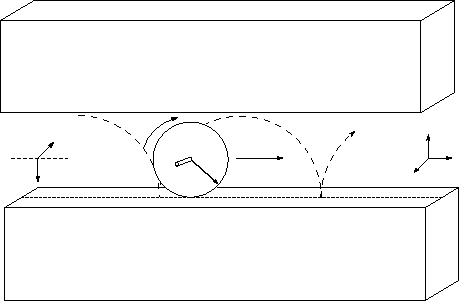
\includegraphics[width=\textwidth]{v3_3}
	\caption{Движение заряда в скрещенных полях}
	\figmark{Crossed fields}
\end{figure}

Для уяснения идеи метода магнетрона, рассмотрим вначале движение заряда в <<плоском магнетроне>>, который можно
представить себе в виде плоского конденсатора, помещённого в магнитное поле так, что $\vec{E}\bot\vec{B}$ (рис.~\figref{Crossed fields}). При этом отрицательная пластина конденсатора играет роль катода, положительная соответственно анода. Если бы магнитного поля не было, то все электроны, вылетевшие без начальной скорости из катода такого плоского диода, попадали бы на анод. При наличии магнитного поля траектории электронов искривляются, вследствие чего при достаточно большом магнитном поле ни один электрон не достигнет анода. Для заданного напряжения между катодом и анодом существует некоторое критическое значение магнитной индукции $B_\text{кр}$, при котором траектории касаются поверхности анода. Если $B<B_\text{кр}$, то все электроны достигают анода и ток через магнетрон имеет то же значение, что и без магнитного поля. Если же $B>B_\text{кр}$, то электроны не достигают анода и ток через лампу равен нулю.

Рассчитаем это критическое значение индукции магнитного поля. Уравнения движения электрона в нашем случае имеет вид
\begin{equation}
	\eqmark{3.9}
	m\frac{dv_x}{dt}=ev_y B,
\end{equation}
\begin{equation}
	\eqmark{3.10}
	m\frac{dv_y}{dt}=eE-ev_x B
\end{equation}
при начальных условиях $x(0)=y(0)=0$, $v_x(0)=v_y(0)=0$.

Непосредственной подстановкой несложно убедиться в том, что решением системы дифференциальных уравнений с заданными
начальными условиями является уравнение циклоиды (в параметрической форме):
\begin{equation}
	\eqmark{3.11}
	x = vt - R\sin\omega t,\qquad y = R(1-\cos\omega t),
\end{equation}
где $ v=E/B$, $R=v/\omega=Em/(eB^2)$.

Касание анода происходит при $2R=d$ ($d$~--- расстояние между анодом и катодом). Этому значению соответствует
критическое поле
\begin{equation}
	B_\text{кр}=\frac{\sqrt{2V}}{d\sqrt{e/m}}.
	\eqmark{3.12}
\end{equation}
Из последней формулы находим удельный заряд:
\begin{equation}
	\eqmark{3.13}
	\frac{e}{m}=\frac{2V}{d^2B_\text{кр}^2}.
\end{equation}

Эта формула позволяет вычислить $e/m$, если при заданном значении напряжения на аноде $V$ найти такое значение
магнитного поля, при превышении которого ток в магнетроне отсутствует.

\labsection{Электрический ток в вакуумном диоде}

Электрический ток в вакуумном диоде представляет собой упорядоченное движение электронов, испускаемых накалённым
катодом. Явление испускания электронов поверхностью твёрдого тела или жидкости называется {\important{электронной эмиссией}}.
Существует несколько видов электронной эмиссии. В частности, в случае испускания электронов поверхностями нагретых тел эмиссия называется {\important{термоэлектронной}}.

Одним из ключевых понятий, лежащих в основе объяснения явления электронной эмиссии, является понятие {\important{работы выхода}}. Под работой выхода понимают работу, которую необходимо совершить для удаления электрона из твёрдого вещества в вакуум в состояние с равной нулю кинетической энергией. В случае термоэлектронной эмиссии работа выхода совершается за счёт кинетической энергии электронов, которой они обладают внутри тела. У чистых металлов работа выхода составляет несколько электрон-вольт.

При повышении температуры металла увеличивается энергия теплового движения электронов, количество быстрых электронов и заметное их количество сможет преодолеть задерживающее электрическое поле и выйти из металла. Если приложить
электрическое поле, направленное к поверхности металла, то оно будет увлекать вышедшие электроны и через вакуум потечёт электрический ток. Этот ток называется {\important{термоэлектронным}}.

При холодном катоде ток через диод при подаче на анод положительного потенциала практически отсутствует. Если же нагреть катод, то в диоде возникает заметный ток. Ток прекращается при изменении полярности батареи. Это как раз и указывает на то, что носителями тока в диоде являются отрицательно заряженные частицы, а именно электроны.

Если бы все электроны, вылетающие из поверхности катода, попадали на анод, то сила термоэлектронного тока $I$ не
зависела бы от величины приложенного напряжения $V$. На самом деле это не так. С возрастанием напряжения ток растёт.
Однако возрастание идёт не пропорционально $V$, так что закон Ома для вакуумного диода не выполняется. При достижении определённого напряжения дальнейшее нарастание тока практически прекращается. Ток достигает предельного значения, называемого током насыщения. Величина тока насыщения определяется количеством электронов, которое способно выйти из поверхности катода в единицу времени, и, следовательно, растёт с ростом температуры. Если электрическое поле настолько сильное, что способно отвести все эмитированные электроны, то дальнейшее увеличение напряжения уже не приводит к увеличению термоэлектронного тока. Этим объясняется явление насыщения тока.

Нелинейная зависимость тока от напряжения объясняется тем, что в пространстве между катодом и анодом образуется
отрицательный пространственный заряд, изменяющий распределение потенциала в диоде.

Допустим, что диод плоский, то есть его электроды представимы в виде двух параллельных плоскостей (расстояние между
электродами много меньше их площади). Направим ось $X$ перпендикулярно к поверхности катода в сторону анода, совместив начало координат с поверхностью катода. В этой модели задача стала одномерной~--- все величины являются функциями только координаты $x$. Потенциал электрического поля $\varphi$ удовлетворяет уравнению Пуассона:
\begin{equation}
	\eqmark{3.14}
	\frac{d^2\varphi}{dx^2}=-\frac{\rho}{\varepsilon_0},
\end{equation}
где $\rho(x)$~--- плотность электрического заряда. Плотность тока $j=\rho v$. Пренебрегая столкновениями электронов, их скорость можно определить из уравнения
\begin{equation*}
	\frac{mv^2}{2}=e\varphi.
\end{equation*}

Начальными тепловыми скоростями, с которыми вылетают электроны с поверхности катода, здесь пренебрегается, а потенциал катода принимается равным нулю. Исключив из этих соотношений плотность электронов и скорость, приходим к уравнению
\begin{equation}
	\eqmark{3.15}
	\frac{d^2\varphi}{dx^2}=\sqrt{\frac{m}{2e\varphi}} j.
\end{equation}

Для однозначного решения этого дифференциального уравнения второго порядка помимо условия $\varphi(0)=0$ необходимо ещё одно граничное условие. Если сопоставить уравнения \eqref{3.14} и \eqref{3.15}, то можно сделать вывод об обращении плотности заряда на катоде в бесконечность. Точка $x=0$ является особой точкой уравнения \eqref{3.15}, в которой оно теряет смысл. Это связано с тем, что мы пренебрегли тепловыми скоростями на катоде, приняв их равными нулю. Оказывается, что в этой модели плотность тока через диод получается конечной, только если напряжённость поля у катода равна нулю. Это условие означает, что поле возникающего вблизи катода пространственного заряда полностью экранирует электрическое поле, создаваемое разностью потенциалов между анодом и катодом. Таким образом, получаем второе граничное условие в виде
\begin{equation*}
	\left.\frac{d\varphi}{dx}\right|_{x = 0}=0.
\end{equation*}

Теперь задача о распределении потенциала становится однозначной и приводит к решению
\begin{equation*}
	j=\frac{4\varepsilon_0}{9x^2}\sqrt{\frac{2e}{m}}\varphi^{3/2}.
\end{equation*}

Так как $\varphi(d)=V$, где $d$~--- расстояние между электродами, то для зависимости тока от напряжения получаем
\begin{equation*}
	I=\frac{4\varepsilon_0 S}{9d^2}\sqrt{\frac{2e}{m}}V^{3/2},
\end{equation*}
где $S$~--- площадь катода. Мы получили зависимость тока через плоский диод от приложенного к нему напряжения, известную как <<закон трёх вторых>> для плоского диода. Оказывается, что не только для плоского вакуумного диода, а и для вакуумного диода с электродами любой другой геометрии ток подчиняется <<закону степени трёх вторых>>.

Полученная формула подсказывает процедуру измерения удельного заряда электрона. Для этого достаточно по
результатам эксперимента построить график зависимости тока от напряжения в степени трёх вторых, который должен
представлять собой прямую линию, проходящую через начало координат. Угол наклона этой прямой линии пропорционален (с известным коэффициентом) квадратному корню из $e/m$~--- искомой величины удельного заряда электрона.

\labsection{Свободные носители заряда в металлах и~полупроводниках. Зонная модель}

Проводимость большинства твёрдых тел связана с движением электронов. Электроны входят в состав атомов всех тел, однако одни тела не проводят электрический ток (диэлектрики), а другие являются хорошими его проводниками. Причина различия заключается в особенностях энергетического состояния внешних электронов атомов в этих веществах.

При объединении атомов в твёрдое тело (кристалл) внешние электроны теряют связь со <<своими>> атомами и теперь принадлежат всему кристаллу в целом. Каждому уровню энергии электрона одиночного атома соответствует в кристалле группа близких по энергии уровней (разрешённая зона), в которой число уровней равно числу мест на соответствующем атомном уровне, умноженному на число атомов в кристалле. Число уровней, объединившихся в зону, при слиянии не меняется. Оно определяет максимальное число электронов, которое может <<поместиться>> в зоне (в силу принципа Паули).

Если одна из энергетических зон до конца заполнена электронами, а следующая зона совершенно пуста, то под действием слабого внешнего электрического поля электронам некуда перетекать, и вещество является \important{диэлектриком}. Верхняя из заполненных зон называется \important{валентной зоной.}

Положение меняется, если в кристалле имеется зона, частично заполненная электронами. В этом случае внешнее электрическое поле может изменить распределение электронов по уровням энергии и создать упорядоченное движение электрических зарядов. Частично заполненная зона называется \important{зоной проводимости}. Частично заполненная электронами зона имеется у всех твёрдых проводников электрического тока; в том числе её имеют все металлы.

Если ширина запрещённой зоны относительно невелика, тепловое движение перебрасывает часть электронов из валентной зоны в свободную~--- зону проводимости. При этом в зоне проводимости появляются электроны, а в валентной зоне~--- свободные места~--- \important{дырки}. Электроны в зоне проводимости и дырки валентной зоны участвуют в переносе заряда. Такие вещества называются \important{полупроводниками}. Обычно к полупроводникам относят материалы с шириной запрещённой зоны $\Delta E \lesssim 2$~эВ. Число носителей тока в полупроводниках экспоненциально увеличивается с~повышением температуры.

Рассматривая коллективное движение электронов почти заполненной зоны, полезно мысленно заполнить свободные места
воображаемыми парами, состоящими из электронов с одинаковыми по величине положительным и отрицательным зарядами. Обычныеотрицательные заряженные электроны заполняют теперь все уровни и, следовательно, не могут принимать участия в проводимости. Они образуют структуру, характерную для изоляторов. Проводимость связана только с введёнными нами
<<электронами>>, обладающими положительным зарядом. Такие <<электроны>> носят название \important{дырок}. При рассмотрении явлений, происходящих в~металлах с~почти заполненной валентной зоной, удобно представлять себе дело так, как если бы проводниками тока были не настоящие электроны, а положительно заряженные дырки. В этом случае говорят о \important{дырочном типе проводимости.}

Электронным типом проводимости обладает большинство чистых металлов. Однако в ряде металлов (бериллий, кадмий и
некоторые другие) основными носителями электрического тока являются дырки. Это связано с особенностями их зонной
структуры.

Рассмотрим прохождение тока в рамках модели свободных электронов.
Закон Ома в дифференциальной форме выражает связь векторов $j$ - плотности тока и $E$ - электрического поля:
\begin{equation}
	j=\lambda E.
	\eqmark{3.16}
\end{equation}

В нулевом магнитном поле, если проводящая среда изотропна (то есть не имеет выделенных направлений), проводимость $\lambda$ является числом (скаляром). Это значит, что векторы $j$ и $E$ сонаправлены. В общем же случае $\widehat{\lambda}$ является тензором второго ранга, то есть матрицей, при умножении которой на вектор $E$ получается вектор $j$. В присутствии магнитного поля эта матрица становится недиагональной в результате эффекта Холла. Тензор удельного сопротивления $\widehat{\rho}$ является обратным к тензору проводимости: $E=\widehat{\rho}j$, то есть $\widehat{\rho}=\widehat{\lambda}^{-1}$.

Электроны в металлах и легированных полупроводниках движутся с большими скоростями во всех направлениях, а под действием тянущего
электрического поля приобретают ненулевую среднюю скорость дрейфового движения $v_{dr}=  Eb$, где $b$ - подвижность.

Разберем магнитосопротивление и эффект Холла на микроуровне. Если магнитное поле направлено вдоль тока, то
оно не влияет на ток, поскольку сила Лоренца равна нулю. Поэтому мы рассмотрим случай, когда поле перпендикулярно
току. Пусть рассматриваемая система для простоты содержит носители только одного сорта (большинство металлов
являются хорошими примерами).
\begin{figure}[h!]
	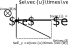
\includegraphics[width=0.9\textwidth]{Chapter_3/Hall_forces}
	\caption{Силы, действующие на носитель заряда в проводящей среде в тянущем электрическом и перпендикулярном ему магнитном полях.}
	\figmark{Hall forces}
\end{figure}

Если в системе локально течет ток электронов $j_x=nev_{dr\, x}$, направленный вдоль оси $x$, а магнитное поле $B$ направлено вдоль оси $z$, то на заряды действует действует сила Лоренца $ F_{L}=e[v_{dr}B]$ вдоль оси $y$.
Сила Лоренца должна приводить к образованию компоненты тока вдоль оси $y$, но по условиям ток течет вдоль $x$. Это значит, что заряды должны перераспределиться таким образом, чтобы полностью скомпенсировать силу
Лоренца, создав в $y$ направлении электрическое холловское поле $E_y=v_{dr}B$. Поскольку сила Лоренца
оказывается полностью скомпенсирована $eE_y$, то электрон движется так, как если бы магнитного поля не
было, то есть $j_x=E_xbne$, $j_y=j_z=0$. Это позволяет написать в явном виде тензор удельного сопротивления:
\begin{equation}
	\widehat{\rho}(B)=\frac{1}{bne}\left(
	\begin{tabular}{ccc}
		{\it 1} & {\it bB} & {\it 0} \\
		{\it -bB} &{\it 1}& {\it 0} \\
		{\it 0} &{\it 0}& {\it 1}\\
	\end{tabular}
	\right).
	\eqmark{3.17}
\end{equation}

Здесь коэффициент, стоящий перед матрицей,
\begin{equation}
	\frac{1}{bne} = \rho_0
	\eqmark{UdSoprot}
\end{equation}
есть удельное сопротивление полупроводника при отсутствии магнитного поля.

Обращением этой матрицы нетрудно получить тензор проводимости:
\begin{equation}
	\widehat{\lambda}(B)=\frac{bne}{1+b^2B^2}\left(
	\begin{tabular}{ccc}
		{\it 1} & {\it bB} & {\it 0} \\
		{\it -bB} &{\it 1}& {\it 0} \\
		{\it 0} &{\it 0}& {\it 1}\\
	\end{tabular}
	\right).
	\eqmark{3.18}
\end{equation}

Существуют две основных и принципиально различных геометрии для исследования магнитосопротивления: геометрия
мостика Холла и геометрия диска Корбино (см. рис.~\figref{Geometries}).

В геометрии мостика Холла ток вынуждают течь вдоль образца, сила Лоренца прибивает носители к краю образца, создавая тем самым холловское поле, которое компенсирует силу Лоренца. Напряжение между точками $V_{xy}$ равно $E_yw$, где, согласно уравнению \eqref{3.17}, $E_y=\rho_{yx}\times j_x=j_x B/(ne)$. Плотность тока, текущего через образец, равна полному току $I$, деленному на площадь поперечного сечения образца $wh$. Таким образом, для холловского напряжения имеем:
\begin{equation}
	V_{xy}=\frac{IB}{neh}.
	\eqmark{3.19}
\end{equation}

В этой же модели для падения напряжения вдоль образца имеем:
\begin{equation}
	V_{xx}=\frac{Il}{nebwh}.
	\eqmark{3.20}
\end{equation}

Tаким образом, удельное сопротивление $\rho_{xx}$ образца не зависит от магнитного поля (магнитосопротивление равно 0). Этот факт объясняется тем, что сила Лоренца и сила ЭДС Холла (рис. \figref{Hall forces}) полностью уравновешивают друг друга. В реальных системах, тем не менее, предположения модели не выполняются и магнитосопротивление зачастую отлично от 0. Причины могут быть различными:
\begin{enumerate}
\item{Система может быть анизотропной, то есть в разных направлениях ($x,y,z$) токопроводящие свойства различны. В этом случае величина силы Лоренца содержит не среднюю дрейфовую скорость, а зависит от направления большой мгновенной скорости электрона.}

\item{Система может быть многокомпонентной. Например, в полупроводниках часто одновременно существуют электроны и дырки, концентрации ($n$ и $p$) и подвижности ($b_n$ и $b_p$) которых в общем случае различаются. Тогда полный тензор проводимости будет суммой тензоров проводимости двух компонент вида \eqref{3.18}. Обращением тензора проводимости в пределе малых магнитных полей можно показать, что холловское сопротивление двухкомпонентной системы в полупроводнике равно:
\begin{equation}
	R_{xy}\equiv \frac{V_{xy}}{I}=\frac{n{b_n}^2-p{b_p}^2}{eh(nb_n+pb_p)^2}B
	\eqmark{3.21}
\end{equation}
}

\item{Существуют квантовые эффекты в проводимости, которые приводят к тому, что подвижность зависит от магнитного поля. Например если сам проводящий материал является ферромагнетиком, то с ростом поля он намагничивается, количество доменов уменьшается, а доменные стенки являются причиной сильного рассеяния, то есть уменьшают подвижность. }
\end{enumerate}

Поскольку холловское сопротивление содержит толщину образца $h$, то договорились называть холловское сопротивление, умноженное на толщину образца, постоянной Холла. Постоянная Холла характеризует материал, так как зависит только от концентрации носителей в нем:
\begin{equation}
	R_x=\frac{1}{ne}
	\eqmark{HallConstant}
\end{equation}
или от соотношений между концентрациями и подвижностями, если в материале несколько типов носителей. В таблице в приложении даны постоянные Холла для различных металлов. Для полупроводников постоянные Холла сильно зависят от наличия малых концентраций примеси и температуры.

Отдельно следует упомянуть, что существуют двумерные системы (например, графен), в которых движение носителей заряда происходит только в плоскости, а движение в перпендикулярном направлении квантовомеханически запрещено. В этих системах концентрация измеряется в количестве носителей на единицу площади, а холловская постоянная есть просто холловское сопротивление, делённое на магнитное поле. В двумерных системах тензоры в формулах \eqref{3.17} и \eqref{3.18} содержат только $x$ и $y$ компоненты, то есть являются матрицами $2\times2$.

Измерения в геометрии мостика Холла представляют собой четырехконтактные измерения, то есть два контакта используются для задания тока через образец, а с двух контактов снимается падение напряжения. Поскольку вольтметр обладает бесконечным сопротивлением (то есть ток через него не течет), измеряемое падение напряжения совершенно не зависит от свойств контактов, а определяется только свойствами материала.

Геометрия диска Корбино представляет собой двухточечную схему, то есть сопротивление образца в ней суммируется с сопротивлениями контактов. Поэтому исключительно важно создать низкоомные контакты к образцу, сопротивлением которых можно пренебречь. В геометрии Корбино из-за аксиальной симметрии не формируется холловское напряжение. Электрическое поле направлено строго по радиусу системы. В магнитном поле ток вынужден протекать под углом к электрическому полю, то есть по спирали. Из-за симметрии полный ток включает только компоненту вдоль радиуса $j_r=\lambda_{xx} E_r$. Плотность тока может быть выражена через полный ток и толщину образца $j_r=I/(2\pi rh)$. Теперь запишем для напряжения:
\begin{equation*}
V={\int_{r_1}}^{r_2}E_r dr={\int_{r_1}}^{r_2}\frac{j_r}{\lambda_{xx}} dr={\int_{r_1}}^{r_2}I\rho_0\frac{1+b^2B^2}{2\pi rh}dr=I\rho_0\frac{1+b^2B^2}{2\pi h}\ln{\frac{r_2}{r_1}}.
\end{equation*}

Если система однокомпонентная, то магнетосопротивление в геометрии Корбино есть
\begin{equation}
	R(B) = R_0(1+b^2B^2)
	\eqmark{MagnetoSoprot}.
\end{equation}

Здесь
\begin{equation}
	R_0 = \frac{\rho_0}{2\pi h} \ln{\frac{r_2}{r_1}}
	\eqmark{KorbinoSoprot}
\end{equation}

Для наблюдения этого магнитосопротивления выбирают систему с большой подвижнотью носителей (как правило, это полупроводник с низкой эффективной массой электронов типа InSb).

\begin{figure}[h!]
	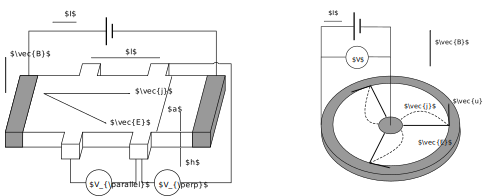
\includegraphics[width=0.9\linewidth]{Chapter_3/2schemes}
	\caption{Две геометрии для исследования влияния магнитного поля на проводящие свойства: мостик Холла (слева) и диск Корбино (справа).}
	\figmark{Geometries}
\end{figure}

При наложении внешнего электрического поля $E$ электроны начинают ускоряться. Однако после некоторого <<свободного пробега>> происходит соударение с решёткой, электрон теряет набранную энергию, и процесс ускорения начинается заново. Соударения с решёткой, подобно вязкому трению, приводят к тому, что результирующее движение электрона можно описать некоторой средней скоростью $\left< v \right> $, пропорциональной внешнему полю:
\begin{equation}
	\eqmark{3.22}
	\left< \vec{v} \right>=-b\vec{E}.
\end{equation}

Введённая здесь величина $b$ называется \important{подвижностью}. В определённых пределах изменения температуры,
напряжённости поля и его частоты эта характеристика вещества остаётся постоянной и приводится в справочниках. Для
положительно заряженных носителей тока в формуле \eqref{3.22}, очевидно, стоит знак <<плюс>>.

При установившемся движении средняя сила, действующая на электроны со стороны кристаллической решётки, равна внешней силе $-eE$ и направлена в противоположную сторону. Поэтому действие кристаллической решётки на движение электронов в среднем эквивалентно силе трения, пропорциональной скорости:
\begin{equation}
	\eqmark{3.23}
	F_\text{тр}=-\frac{e}{b}\average{\vec{v}}.
\end{equation}

Если концентрация электронов равна $n$, величина плотности тока определится очевидным соотношением
\begin{equation}
	\eqmark{3.24}
	j=en\average{v}=enbE.
\end{equation}

Таким образом, выполняется закон Ома~--- величина плотности тока $j$ пропорциональна напряжённости поля $E$:
\begin{equation}
	\eqmark{3.25}
	j=\sigma E.
\end{equation}

Сравнивая \eqref{3.24} и \eqref{3.25}, получаем выражение для проводимости
\begin{equation}
	\eqmark{3.26}
	\sigma=enb.
\end{equation}

Химически чистые полупроводники обладают проводимостью, которая связана с небольшим числом электронов в зоне
проводимости и таким же числом дырок в валентной зоне. Такая проводимость называется собственной~--- она не связана с примесями. Добавление небольшого количества специально подобранных примесей (так называемое
легирование) может существенно увеличить проводимость полупроводников или даже создать ощутимую проводимость при комнатной температуре в веществах с запрещённой зоной, ширина которой заметно превышает 2~эВ. Такое происходит, когда атомы примеси имеют энергетические уровни в запрещённой зоне основного материала.

Если заполненные примесные уровни расположены вблизи потолка запрещённой зоны, находящиеся на этих уровнях электроны легко переходят в зону проводимости. Наоборот, на свободные уровни у дна зоны проводимости легко переходят электроны валентной зоны с образованием в этой зоне дополнительного количества дырок. В обоих случаях число переносчиков заряда увеличивается, и проводимость возрастает. В первом случае говорят о полупроводниках \important{электронного}, или $n$-типа, а во втором~--- о  полупроводниках дырочного, или $p$-типа. В общем случае в процессе электрической проводимости участвуют как электроны, так и дырки. Удельная электрическая проводимость полупроводника при этом равна
\begin{equation}
	\eqmark{3.27}
	\sigma=e(nb_e+pb_p),
\end{equation}
где $n$ и $p$~--- концентрации электронов и дырок, а $b_e$ и $b_p$~--- их подвижности. В случае \important{примесной
проводимости} один тип носителей обычно существенно преобладает над другим и в формуле \eqref{3.27} можно пренебречь одним из слагаемых.



\begin{lab:literature}
	\item{ \emph{Сивухин Д.В.} Общий курс физики.~--- T.~III. Электричество.~--- М.: Наука, 1983. \S\S~86, 95, 98, 100.}
	\item{ \emph{Кингсеп А.С., Локшин Г.Р., Ольхов О.А.} Основы физики. Т.~1.~--- М.: Физматлит, 2001. \S\S~8.1--8.3.}
\end{lab:literature}


